
\subsection{Арифметическое кодирование}
\textbf{Арифметическое кодирование} является улучшенной версией кода Хаффмана, потому что позволяет кодировать символы нецелым числом бит. Алгоритм кодирования устроен так:
\begin{enumerate}
    \item Начните работу с отрезка от 0 до 1.
    \item Поделите отрезок на части в соотношении, равном отношению частот символов
    \item В зависимости от текущего символа в кодируемой строке перейдите к нужному отрезку
    \item Если строка не кончилась перейдите к пункту 2, иначе выберите на полученном отрезке точку вида $\frac{p}{2^q}$ с наименьшим $q$, вашим кодом будет двоичный вектор длины $q$, в котором записано число $p$
\end{enumerate}
\begin{center}
  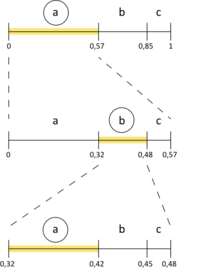
\includegraphics[height=9.1cm]{assets/arif1.png}
\end{center}
Декодирование работает точно так же, мы снова делим отрезок на подотрезки, но теперь мы уже знаем в какой из них нам нужно, так как мы знаем точку, которая ответу принадлежит, перейдем в нужный отрезок и продолжим алгоритм.
\begin{center}
  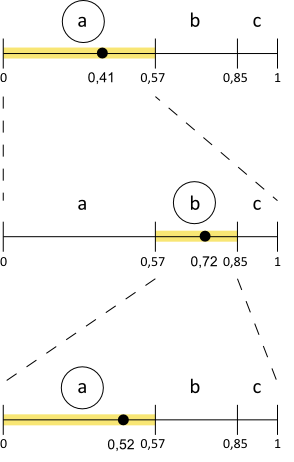
\includegraphics[height=9.1cm]{assets/arif2.png}
\end{center}
\subsection{LZW}
Алгоритм $LZW$ - алгоритм для сжимания данных, основанный на поиске повторяющихся кусков данных и сжимания их. Для сохранения данных о закономерностях предлагается использования буфера. В общем виде алгоритм действия такой:
\begin{enumerate}
    \item Добавление всех символов алфавита в буфер с наименьшими номерами
    \item Инициализируем скользящее окно $X$ как пустую строку
    \item Обработка очередной символа $S$ из текста.
    \item Если $S$ — это символ конца сообщения, то выдать код для $X$, иначе:
    \subitem 4.1. Фраза $XS$ есть в словаре:
    Приписать к $X$ символ $S$, \\Перейти к шагу 3.
    \subitem 4.2 Фразы $XS$ нет в словаре:
    Выдать код для входной фразы $X$, добавить $XY$ в словарь и присвоить $X$ значение $S$. Перейти к Шагу 3. 
\end{enumerate}

Алгоритм декодирования:
\begin{enumerate}
    \item Все возможные символы заносятся в словарь. В скользящее окно $X$
    заносится первый код декодируемого сообщения.
    \item  Считать очередной код $S$ из сообщения.
    \item Если $S$ — это конец сообщения, то выдать символ, соответствующий коду $X$, иначе:
    \subitem 3.1 Если фразы под кодом $XS$ нет в словаре, вывести фразу, соответствующую коду $X$, а фразу с кодом $XS$
    занести в словарь.
    \subitem 3.2 Иначе присвоить входной фразе код $XS$ и перейти к Шагу 2 .
\end{enumerate}
\subsection{Алгоритм Барроуза-Уиллера}
Алгоритм Барроуза-Уиллера также как и $LZW$ производит поиск паттернов в данных, но вместо того, чтобы сжимать их, он просто превращает их в последовательности из одинаковых символов для увеличения эффективности дальнейшего сжатия. Работает он так:
\begin{enumerate}
    \item Выписываем все циклические сдвиги данных в отсортированном порядке.
    \item В качестве результата берем последний столбец, для декодирования запоминаем, какой из символов этого столбца является символом исходной строки.
\end{enumerate} 
\begin{center}
  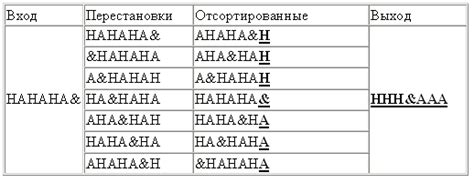
\includegraphics[height=4cm]{assets/barr.jpg}
\end{center}
\textbf{Почему так происходит:} Предположим у нас есть паттерн $s$, который встречается много раз в исходной строке. Тогда если мы возьмем и отрежем у этого паттерна первый символ, пусть он будет $a$, тогда в тех случаях, когда этот символ будет в конце циклического сдвига, остальная часть паттерна будет в его начале, а значит, с большой вероятностью, эти символы будут идти подряд.

Декодирование будет устроено так:
\begin{enumerate}
    \item Изначально у нас будет записан только результат кодирования, который мы отсортируем
    \item Приписываем к полученной таблице слева результат кодирования и сортируем
    \item Если таблица не готова, то перейти к шагу 2, иначе мы берем строку.
\end{enumerate}
Это декодирование основано на том, что у нас выписаны все циклические сдвиги, а значит на самом деле переход от $i$ого столбца к $i+1$ому это какая-то перестановка, причем перестановка постоянная. Тогда эту перестановку можно получить если перебросить первый столбец в конец, у нас получится пара - отсортированный столбец и наш результат левее, значит если так повторять, то мы просто будем применять эту перестановку и получать предыдущий столбец. Сложность декодирования выходит $O(n^2\log n)$.

Но если мы 1 раз построим перестановку и будем применять ее только к элементу последнего столбца, который принадлежит искомой строке, то мы можем восстановить закодированные данные без восстановления всей таблицы, что будет работать уже за $n\log n$.
